\begin{figure}[t]
\centering
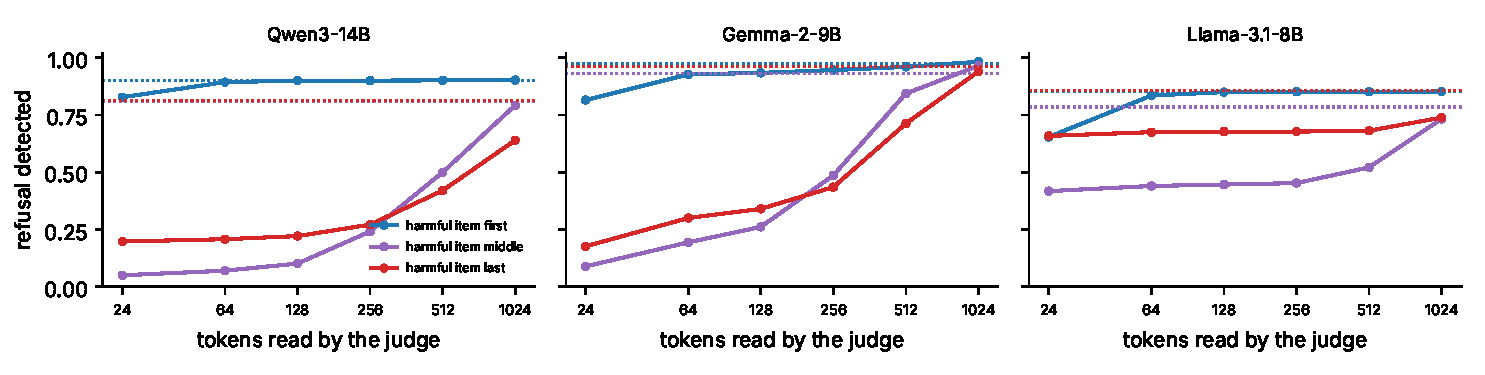
\includegraphics[width=\linewidth]{fig_horizon.pdf}
\caption{Refusal detected by a judge that reads only the first $N$ generated tokens and looks for any refusal
phrase, for harmful items placed first, in the middle or last (numbered template, $k\ge3$; 800 responses per
line). Dotted lines: target refusal in the full response.}
\label{fig:horizon}
\end{figure}

\paragraph{How far must a judge read?} \Cref{fig:horizon} varies the number of tokens a refusal-phrase judge
reads. When the harmful item comes first, 64 tokens recover nearly all refusals for every model. When it comes in the middle,
Qwen3-14B's detected refusal rises from 5\% at 24 tokens to 24\% at 256, 50\% at 512 and 79\% at 1{,}024,
against 81\% in the full response. Gemma-2-9B follows the same course (9\%, 49\%, 84\%, 96\%). Judges that read
a few hundred tokens, a common budget in jailbreak evaluations, therefore still miss most deferred refusals in
lists of four or more items.

\paragraph{Where models refuse.} The curves differ by model because models refuse in different places. When
the harmful item is not first, Qwen3-14B places \QwenInItemShare\ of its refusals \emph{in the item}: it answers
the preceding benign items, then declines. Gemma-2-9B does so in \GemmaInItemShare\ of cases. Llama-3.1-8B
reverses the pattern and refuses \emph{up front} in \LlamaUpfrontShare\ of cases (``I can't help with request 4,
but here are the others''). Its detected refusal is therefore nearly flat in $N$, and a 24-token judge already
sees most of it. A fixed short horizon thus does not just add noise; it ranks models by \emph{where} they refuse
rather than \emph{whether} they do. Under a 24-token judge, Llama-3.1-8B looks far safer than Qwen3-14B on list
prompts (\LlamaMiddleVone\ vs.\ \QwenMiddleVone\ refusal, middle position), although its full-response ASR is
higher (\LlamaMiddleASR\ vs.\ \QwenMiddleASR).
